% =====================================================================
%  Successioni di funzioni -- capitolo 1
% =====================================================================

\section{Successioni di funzioni}

\subsection{Motivazione: da Taylor alle serie di funzioni}

Sia $I \subseteq \mathbb{R}$ un intervallo, $x_0 \in I$ e $f \in C^\infty(I)$.
Poiché $f$ è derivabile quante volte si vuole, per \emph{ogni} $n \in \mathbb{N}$
possiamo scrivere il polinomio di Taylor di ordine $n$ centrato in $x_0$:
\[
\begin{aligned}
  P_n(x) &= \sum_{k=0}^{n} \frac{f^{(k)}(x_0)}{k!}\,(x-x_0)^k \\
         &= f(x_0) + f'(x_0)(x-x_0) + \frac{f''(x_0)}{2!}(x-x_0)^2 + \dots
            + \frac{f^{(n)}(x_0)}{n!}(x-x_0)^n .
\end{aligned}
\]

In Analisi~I lo abbiamo usato nella \textbf{formula di Taylor con resto di Peano}:
\[
  f(x) \;=\; P_n(x) + o\big((x-x_0)^n\big) \qquad \text{per } x \to x_0 .
\]
Qui $n$ è \emph{fissato} e l'informazione è solo \emph{locale}: vale vicino a $x_0$.

Ora ci chiediamo cosa succede se lasciamo crescere $n$ senza limite, cioè se ha
senso scrivere
\[
  f(x) \;=\; \sum_{k=0}^{\infty} \frac{f^{(k)}(x_0)}{k!}\,(x-x_0)^k
  \;=\; a_0 + a_1 (x-x_0) + a_2 (x-x_0)^2 + \dots ,
  \qquad a_k = \frac{f^{(k)}(x_0)}{k!} .
\]
Il membro destro è una \textbf{somma infinita di funzioni}, cioè una
\textbf{serie di funzioni}. Come per le serie numeriche, la sua somma va intesa
come limite delle somme parziali:
\[
  \sum_{k=0}^{\infty} \frac{f^{(k)}(x_0)}{k!}\,(x-x_0)^k
  \;:=\; \lim_{n \to +\infty} P_n(x) .
\]
Le somme parziali $P_0, P_1, P_2, \dots$ però non sono numeri, sono
\emph{funzioni}. Per dare senso a questo limite serve prima capire cosa vuol dire
che una \textbf{successione di funzioni} converge: è l'argomento di questo capitolo.

\BoxBlue{Attenzione}{}{%
  $f \in C^\infty$ garantisce che la serie di Taylor si possa \emph{scrivere},
  ma \textbf{non} che converga a $f$. Ad esempio
  \[
    f(x) =
    \begin{cases}
      e^{-1/x^2} & x \neq 0 \\[2pt]
      0          & x = 0
    \end{cases}
  \]
  è $C^\infty(\mathbb{R})$ con $f^{(k)}(0) = 0$ per ogni $k$: la sua serie di
  Taylor in $0$ è identicamente nulla, mentre $f(x) > 0$ per $x \neq 0$.
  Le funzioni che coincidono con la propria serie di Taylor si dicono
  \textbf{analitiche}.
}

\subsection{Definizione}

\BoxBlue{Richiamo (successione numerica)}{}{%
  Una successione numerica è una legge che a ogni $n \in \mathbb{N}$ associa
  un numero reale:
  \[
    n \longmapsto a_n \in \mathbb{R} .
  \]
}

\BoxGreen{Definizione (successione di funzioni)}{}{%
  Sia $I \subseteq \mathbb{R}$. Una \textbf{successione di funzioni} definite in
  $I$ è una legge che a ogni $n \in \mathbb{N}$ associa una funzione
  \[
    n \longmapsto f_n : I \to \mathbb{R} .
  \]
  Si indica con $(f_n)_{n \in \mathbb{N}}$ o semplicemente $(f_n)$.
}

L'insieme di definizione $I$ va \textbf{sempre} indicato: come vedremo, il
comportamento della successione dipende fortemente da $I$.

\BoxBlue{Osservazione}{}{%
  L'espressione $f_n(x)$ dipende da \textbf{due variabili indipendenti},
  $n \in \mathbb{N}$ e $x \in I$:
  \begin{itemize}
    \item fissato $n$, si ottiene una \emph{funzione} $x \mapsto f_n(x)$;
    \item fissato $x \in I$, si ottiene una \emph{successione numerica}
          $n \mapsto f_n(x)$.
  \end{itemize}
  Il secondo punto è quello che ci permetterà di riusare quanto sappiamo sui
  limiti di successioni numeriche.
}

\paragraph{Esempio 1.} Consideriamo
\[
  f_n(x) = \frac{x}{n}, \qquad x \in \mathbb{R} .
\]

\emph{Fissando $n$} otteniamo le funzioni
\[
  f_1(x) = x, \qquad f_2(x) = \frac{x}{2}, \qquad f_3(x) = \frac{x}{3},
  \qquad \dots
\]
cioè rette per l'origine con pendenza $1/n$.

\emph{Fissando $x$} otteniamo successioni numeriche:
\[
  x = 1: \quad f_n(1) = \frac{1}{n},
  \qquad\qquad
  x = 2: \quad f_n(2) = \frac{2}{n},
  \qquad\qquad
  x \text{ generico}: \quad f_n(x) = \frac{x}{n} .
\]
Per ogni $x$ fissato vale $f_n(x) \to 0$: nella prossima sezione vedremo come
questo si legge sul grafico e come formalizzarlo.

% ---------------------------------------------------------------------
\subsection{Rappresentazione grafica}

Disegnando sullo stesso piano i grafici di $f_1, f_2, f_3, \dots$ otteniamo un
\emph{fascio di grafici}. Per $f_n(x) = x/n$ sono rette per l'origine che, al
crescere di $n$, si adagiano sull'asse $x$.

\begin{figure}[H]
\centering
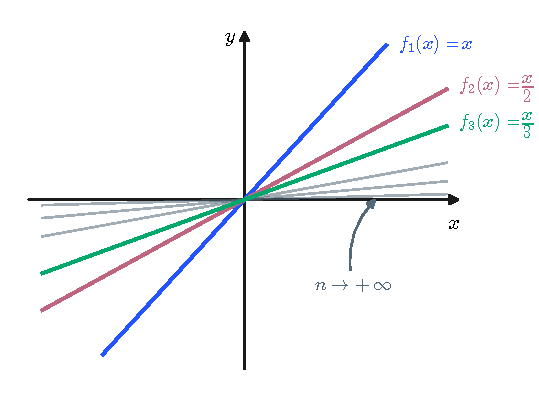
\includegraphics[width=0.78\textwidth]{immagini/succ_fascio_rette}
\caption{Le funzioni $f_n(x) = x/n$: al crescere di $n$ le rette si schiacciano
sull'asse $x$.}
\end{figure}

Il grafico suggerisce che le $f_n$ ``tendono'' alla funzione costante
\[
  f(x) = 0 .
\]
Dobbiamo dare un significato preciso a questa affermazione.

% ---------------------------------------------------------------------
\subsection{Convergenza puntuale}

\BoxBlue{Richiamo (limite di una successione numerica)}{}{%
  \[
    \lim_{n \to +\infty} a_n = \ell \in \mathbb{R}
    \iff
    \forall \varepsilon > 0 \;\; \exists\, \nu_\varepsilon \in \mathbb{N} :
    \;\; |a_n - \ell| < \varepsilon \quad \forall n > \nu_\varepsilon .
  \]
}

L'idea più naturale è fissare $x \in I$ e applicare questa definizione alla
successione numerica $n \mapsto f_n(x)$.

\BoxGreen{Definizione (convergenza puntuale)}{}{%
  Siano $f_n : I \to \mathbb{R}$ e $f : I \to \mathbb{R}$. Diciamo che $(f_n)$
  \textbf{converge puntualmente} a $f$ in $I$ se
  \[
    \lim_{n \to +\infty} f_n(x) = f(x) \qquad \forall x \in I .
  \]
  La funzione $f$ si chiama \textbf{limite puntuale} della successione.
}

Esplicitando il limite, la definizione diventa
\[
  \forall x \in I \;\; \forall \varepsilon > 0 \;\; \exists\, \nu_{\varepsilon,x} \in \mathbb{N} :
  \;\; |f_n(x) - f(x)| < \varepsilon \quad \forall n > \nu_{\varepsilon,x} .
\]
L'indice $\nu_{\varepsilon,x}$ dipende \textbf{sia da $\varepsilon$ sia da $x$}:
in punti diversi la successione può avvicinarsi al limite con velocità molto
diverse. Questo dettaglio sarà il cuore della sezione~\ref{sec:unif}.

\paragraph{Notazione.} Si scrive indifferentemente
\[
  \lim_{n \to +\infty} f_n(x) = f(x) \;\; \forall x \in I
  \qquad \text{oppure} \qquad
  f_n \xrightarrow{\;p\;} f \;\; \text{in } I .
\]
Il limite è sempre fatto per $n \to +\infty$, con $x$ fissato: la variabile $x$
\emph{non} va da nessuna parte.

% ---------------------------------------------------------------------
\subsection{Calcolo del limite puntuale: esempi}

Il metodo è sempre lo stesso: si fissa $x$, si calcola il limite in $n$ e si
controlla se esistono valori di $x$ per cui il calcolo cambia.

\paragraph{Esempio 1 (ripreso).}
\[
  f_n(x) = \frac{x}{n}, \qquad x \in \mathbb{R}.
\]
Per ogni $x$ fissato il numeratore è costante e il denominatore diverge, quindi
\[
  f_n \xrightarrow{\;p\;} f \equiv 0 \quad \text{in } \mathbb{R} .
\]

\paragraph{Esempio 2.}
\[
  f_n(x) = \frac{n + x}{n + (-1)^n \sqrt{n}}, \qquad x \in \mathbb{R}, \;\; n \ge 2
\]
(per $n = 1$ il denominatore si annulla). Dividendo numeratore e denominatore
per $n$:
\[
  f_n(x) = \frac{1 + \dfrac{x}{n}}{1 + \dfrac{(-1)^n}{\sqrt{n}}}
  \;\longrightarrow\; \frac{1 + 0}{1 + 0} = 1 ,
\]
quindi
\[
  f_n \xrightarrow{\;p\;} f \equiv 1 \quad \text{in } \mathbb{R} .
\]

\paragraph{Esempio 3.}
\[
  f_n(x) = \frac{n}{n^2 x + 2n - 1} .
\]
Qui il termine dominante del denominatore è $n^2 x$, che però \textbf{sparisce
se $x = 0$}: i due casi vanno trattati separatamente.
\begin{itemize}
  \item Se $x \neq 0$, dividendo per $n$:
  \[
    f_n(x) = \frac{1}{n x + 2 - \dfrac{1}{n}} \longrightarrow 0 ,
    \qquad \text{perché } |n x| \to +\infty .
  \]
  \item Se $x = 0$:
  \[
    f_n(0) = \frac{n}{2n - 1} \longrightarrow \frac{1}{2} .
  \]
\end{itemize}
Quindi
\[
  f_n \xrightarrow{\;p\;} f(x) =
  \begin{cases}
    0           & x \neq 0 \\[2pt]
    \dfrac{1}{2} & x = 0
  \end{cases}
  \qquad \text{in } \mathbb{R} .
\]

\BoxBlue{Osservazione}{}{%
  $f_n$ non è definita dove $n^2 x + 2n - 1 = 0$. Per $x$ fissato, però, questa
  è un'equazione di secondo grado in $n$ e ha al più due soluzioni: da un certo
  $n$ in poi $f_n(x)$ è definita e il limite ha senso.

  Morale: bisogna sempre guardare \emph{come interagiscono} $x$ e $n$. I valori
  di $x$ che annullano il termine dominante vanno studiati a parte.
}

\paragraph{Esempio 4.}
\[
  f_n(x) = x^n, \qquad x \in [0,1] .
\]
Per $0 \le x < 1$ si ha $x^n \to 0$, mentre per $x = 1$ si ha $1^n = 1$. Quindi
\[
  f_n \xrightarrow{\;p\;} f(x) =
  \begin{cases}
    0 & 0 \le x < 1 \\[2pt]
    1 & x = 1
  \end{cases}
  \qquad \text{in } [0,1] .
\]

\begin{figure}[H]
\centering
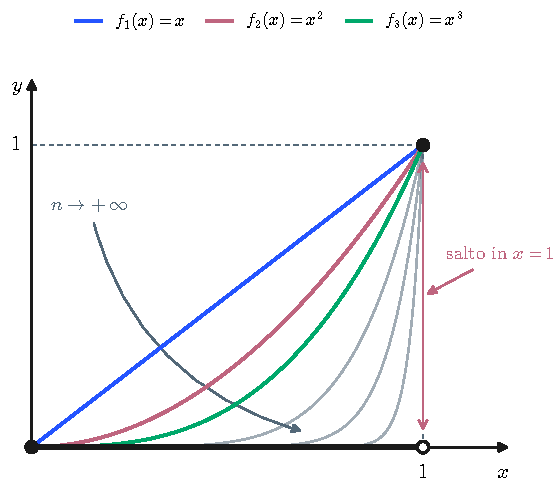
\includegraphics[width=0.62\textwidth]{immagini/succ_xn_puntuale}
\caption{$f_n(x) = x^n$ su $[0,1]$. In nero il limite puntuale: vale $0$ su
$[0,1[$ e salta a $1$ in $x = 1$.}
\end{figure}

\paragraph{Esempio 5.}
\[
  f_n(x) = x^{1/n} = \sqrt[n]{x}, \qquad x \in [0,1] .
\]
Per $x \in \,]0,1]$ si ha $x^{1/n} \to x^0 = 1$, mentre $f_n(0) = 0$ per ogni $n$.
Quindi
\[
  f_n \xrightarrow{\;p\;} f(x) =
  \begin{cases}
    0 & x = 0 \\[2pt]
    1 & 0 < x \le 1
  \end{cases}
  \qquad \text{in } [0,1] .
\]

\begin{figure}[H]
\centering
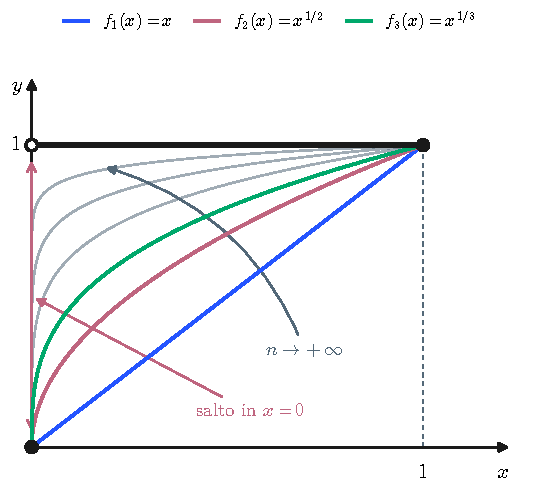
\includegraphics[width=0.62\textwidth]{immagini/succ_x1n_puntuale}
\caption{$f_n(x) = x^{1/n}$ su $[0,1]$. In nero il limite puntuale: vale $1$ su
$]0,1]$ e salta a $0$ in $x = 0$.}
\end{figure}

% ---------------------------------------------------------------------
\subsection{I limiti della convergenza puntuale}

\BoxBlue{Osservazione}{}{%
  Negli esempi 4 e 5 le $f_n$ sono tutte continue (le $x^n$ sono addirittura
  $C^\infty$), ma il limite puntuale \textbf{non è nemmeno continuo}.
  La convergenza puntuale, quindi, non conserva la continuità, e a maggior
  ragione non conserva la derivabilità.
}

Questo è un problema serio per il nostro obiettivo: vogliamo scrivere funzioni
come limiti di polinomi e continuare a lavorarci sopra (derivarle, integrarle).
Serve una \textbf{nozione di convergenza più forte}, che trasmetta al limite le
buone proprietà delle $f_n$.

Mettiamo a confronto i tre esempi principali visti finora.

\begin{figure}[H]
\centering
\begin{minipage}{0.32\textwidth}\centering
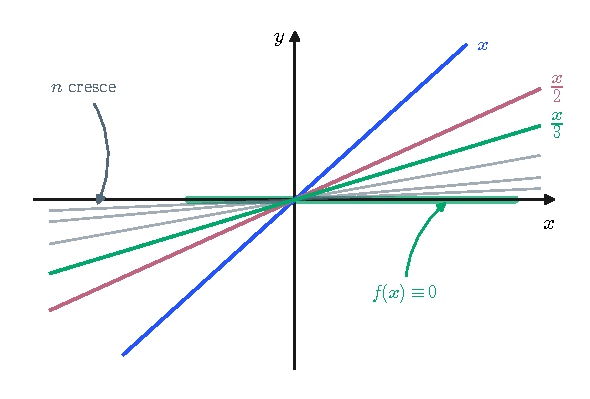
\includegraphics[width=\linewidth]{immagini/unif_fascio_rette}\\[2pt]
{\small $\dfrac{x}{n}$ in $\mathbb{R}$: limite $f \equiv 0$, continuo}
\end{minipage}\hfill
\begin{minipage}{0.32\textwidth}\centering
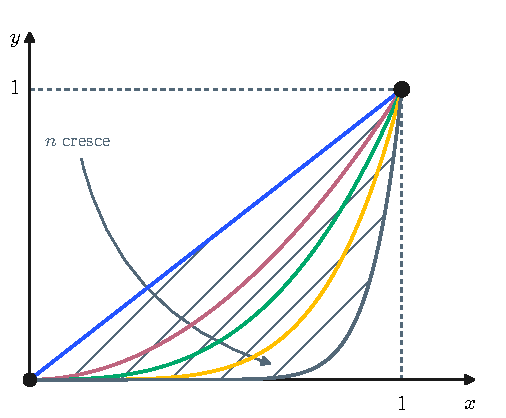
\includegraphics[width=\linewidth]{immagini/unif_xn_tratteggio}\\[2pt]
{\small $x^n$ in $[0,1]$: limite discontinuo in $x = 1$}
\end{minipage}\hfill
\begin{minipage}{0.32\textwidth}\centering
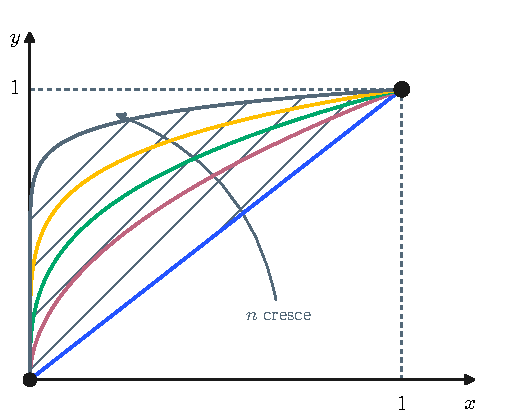
\includegraphics[width=\linewidth]{immagini/unif_x1n_tratteggio}\\[2pt]
{\small $x^{1/n}$ in $[0,1]$: limite discontinuo in $x = 0$}
\end{minipage}
\caption{I tre esempi a confronto. In nero, il limite puntuale.}
\end{figure}

Nel primo caso il limite è continuo, negli altri due no. Vedremo però che anche
nel primo caso la convergenza ha un difetto: le rette si avvicinano all'asse $x$
sempre più lentamente man mano che $|x|$ cresce.

% ---------------------------------------------------------------------
\subsection{Convergenza uniforme}\label{sec:unif}

Il difetto della convergenza puntuale sta nel fatto che $\nu_{\varepsilon,x}$
dipende da $x$. Negli esempi 4 e 5, più ci si avvicina al punto di salto, più
$n$ deve essere grande per avere $|f_n(x) - f(x)| < \varepsilon$. Chiediamo
allora che uno stesso indice funzioni \emph{per tutti} gli $x$.

\BoxGreen{Definizione (convergenza uniforme)}{}{%
  Siano $f_n : I \to \mathbb{R}$ e $f : I \to \mathbb{R}$. Diciamo che $(f_n)$
  \textbf{converge uniformemente} a $f$ in $I$, e scriviamo
  $f_n \rightrightarrows f$ in $I$, se
  \[
    \forall \varepsilon > 0 \;\; \exists\, \nu_\varepsilon \in \mathbb{N} :
    \;\; |f_n(x) - f(x)| < \varepsilon \quad \forall n > \nu_\varepsilon, \;\; \forall x \in I .
  \]
}

Conviene confrontare le due definizioni: cambia solo \textbf{la posizione di
``$\forall x$''}.
\[
\begin{aligned}
  \text{puntuale:} \quad & \forall x \in I \;\; \forall \varepsilon > 0 \;\; \exists\, \nu_{\varepsilon,x} : \;\; |f_n(x) - f(x)| < \varepsilon \;\; \forall n > \nu_{\varepsilon,x} \\[4pt]
  \text{uniforme:} \quad & \forall \varepsilon > 0 \;\; \exists\, \nu_{\varepsilon} : \;\; |f_n(x) - f(x)| < \varepsilon \;\; \forall n > \nu_{\varepsilon}, \;\; \forall x \in I
\end{aligned}
\]
Nel primo caso $x$ viene scelto \emph{prima} di $\nu$, che quindi può dipenderne;
nel secondo $\nu$ viene scelto prima di $x$ e deve andare bene per tutti.

\paragraph{Interpretazione grafica.} La condizione
$|f_n(x) - f(x)| < \varepsilon$ per ogni $x \in I$ significa
\[
  f(x) - \varepsilon < f_n(x) < f(x) + \varepsilon \qquad \forall x \in I ,
\]
cioè il grafico di $f_n$ sta tutto dentro il ``tubo'' di raggio $\varepsilon$
attorno al grafico di $f$. La convergenza è uniforme se, comunque si scelga lo
spessore $\varepsilon$ del tubo, da un certo indice in poi \emph{tutti} i grafici
delle $f_n$ ci stanno dentro.

\begin{figure}[H]
\centering
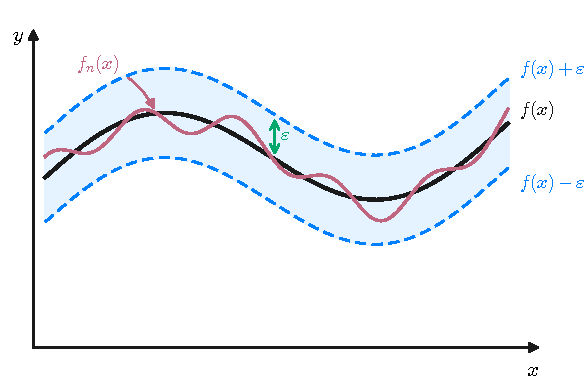
\includegraphics[width=0.88\textwidth]{immagini/tubo_epsilon}
\caption{Per $n > \nu_\varepsilon$ il grafico di ogni $f_n$ è contenuto nel tubo
di raggio $\varepsilon$ attorno a $f$.}
\end{figure}

% ---------------------------------------------------------------------
\subsection{Caratterizzazione con l'estremo superiore}

Verificare la definizione ``a mano'' è scomodo. Si usa quasi sempre questa
forma equivalente. Per ogni $n$ poniamo
\[
  M_n := \sup_{x \in I} |f_n(x) - f(x)| \;\in [0, +\infty] .
\]
Fissato $n$, $M_n$ è un \emph{numero}: la massima distanza verticale tra i
grafici di $f_n$ e $f$. Quindi $(M_n)$ è una \emph{successione numerica}.

\BoxGreen{Teorema (caratterizzazione della convergenza uniforme)}{}{%
  \[
    f_n \rightrightarrows f \;\; \text{in } I
    \iff
    \lim_{n \to +\infty} \, \sup_{x \in I} |f_n(x) - f(x)| = 0 .
  \]
}

\noindent\textit{Dimostrazione.}
($\Rightarrow$) Fissato $\varepsilon > 0$, per $n > \nu_\varepsilon$ vale
$|f_n(x) - f(x)| < \varepsilon$ per ogni $x \in I$. Passando all'estremo
superiore
\[
  M_n \le \varepsilon \qquad \forall n > \nu_\varepsilon ,
\]
(il $<$ diventa $\le$, ma per l'arbitrarietà di $\varepsilon$ non cambia nulla),
quindi $M_n \to 0$.

($\Leftarrow$) Se $M_n \to 0$, fissato $\varepsilon > 0$ esiste
$\nu_\varepsilon$ tale che $M_n < \varepsilon$ per $n > \nu_\varepsilon$. Allora,
per ogni $x \in I$,
\[
  |f_n(x) - f(x)| \le M_n < \varepsilon \qquad \forall n > \nu_\varepsilon . \qquad \square
\]

\paragraph{Ricetta operativa.}
\begin{enumerate}
  \item Si calcola il limite puntuale $f$.
  \item Si calcola $M_n = \sup_I |f_n - f|$, di solito studiando la funzione
        $x \mapsto |f_n(x) - f(x)|$ con le derivate (ricerca di massimi e
        minimi, con $n$ trattato come parametro).
  \item Si verifica se $M_n \to 0$.
\end{enumerate}

% ---------------------------------------------------------------------
\needspace{8\baselineskip}
\subsection{Uniforme implica puntuale}

\BoxGreen{Proposizione}{}{%
  Se $f_n \rightrightarrows f$ in $I$, allora $f_n \xrightarrow{\;p\;} f$ in $I$.
}

\noindent\textit{Dimostrazione.} Fissati $x \in I$ ed $\varepsilon > 0$, basta
prendere $\nu_{\varepsilon,x} := \nu_\varepsilon$. \hfill $\square$

\medskip
Il viceversa è \textbf{falso}, come mostrano gli esempi seguenti. Di conseguenza,
l'unico candidato possibile come limite uniforme è il limite puntuale: per
questo si calcola sempre prima quello.

% ---------------------------------------------------------------------
\subsection{Esempi}

\paragraph{Esempio 1 (ripreso): $f_n(x) = x/n$.} Sappiamo che $f_n \to 0$
puntualmente in $\mathbb{R}$.
\begin{itemize}
  \item \emph{In $\mathbb{R}$:}
  \[
    M_n = \sup_{x \in \mathbb{R}} \left| \frac{x}{n} - 0 \right|
        = \frac{1}{n} \sup_{x \in \mathbb{R}} |x| = +\infty \qquad \forall n ,
  \]
  quindi la convergenza \textbf{non} è uniforme in $\mathbb{R}$. Notare che il
  limite $f \equiv 0$ è continuo: un limite continuo \emph{non} garantisce
  la convergenza uniforme.
  \item \emph{In $[-a, a]$, con $a > 0$:}
  \[
    M_n = \frac{1}{n} \sup_{x \in [-a,a]} |x| = \frac{a}{n} \longrightarrow 0 ,
  \]
  quindi la convergenza è uniforme. Poiché ogni insieme limitato è contenuto in
  un intervallo del tipo $[-a,a]$, c'è convergenza uniforme su \textbf{ogni
  insieme limitato}.
\end{itemize}

\paragraph{Esempio 4 (ripreso): $f_n(x) = x^n$.}
\begin{itemize}
  \item \emph{In $[0,1]$:} in $x = 1$ la differenza è nulla, quindi
  \[
    M_n = \sup_{x \in [0,1[} x^n = 1 \qquad \forall n
  \]
  (è un estremo superiore, non un massimo). Dato che $M_n = 1 \not\to 0$, la
  convergenza \textbf{non} è uniforme.
  \item \emph{In $[0,1[$:} il conto è identico, $M_n = 1$. Togliere il punto
  $x = 1$ non basta: il problema è tutto l'\emph{intorno} di $1$.
  \item \emph{In $[0,b]$, con $0 < b < 1$:} $x^n$ è crescente, quindi
  \[
    M_n = \sup_{x \in [0,b]} x^n = b^n \longrightarrow 0 ,
  \]
  e la convergenza è uniforme. Per ottenerla bisogna \textbf{allontanarsi dal
  punto di discontinuità} del limite.
\end{itemize}

\paragraph{Esempio 5 (ripreso): $f_n(x) = x^{1/n}$.} La situazione è
speculare.
\begin{itemize}
  \item \emph{In $[0,1]$:} in $x = 0$ la differenza è nulla, e su $]0,1]$ vale
  $|x^{1/n} - 1| = 1 - x^{1/n}$, quindi
  \[
    M_n = \sup_{x \in ]0,1]} \big(1 - x^{1/n}\big) = 1 \qquad \forall n ,
  \]
  perché $x^{1/n} \to 0$ per $x \to 0^+$. Non c'è convergenza uniforme.
  \item \emph{In $[a,1]$, con $0 < a < 1$:} $1 - x^{1/n}$ è decrescente in $x$,
  quindi il sup è assunto in $x = a$:
  \[
    M_n = 1 - a^{1/n} \longrightarrow 1 - 1 = 0 ,
  \]
  e la convergenza è uniforme.
\end{itemize}

\BoxBlue{Osservazione}{}{%
  Negli esempi 4 e 5 le $f_n$ sono continue, il limite no, e la convergenza non
  è uniforme. Non è un caso: la convergenza uniforme è proprio la nozione
  ``più forte'' che cercavamo, e vedremo che conserva la continuità.
}

% ---------------------------------------------------------------------
\subsection{Esercizio svolto}

\paragraph{Testo.} Studiare la convergenza puntuale e uniforme di
\[
  f_n(x) = \frac{x}{1 + n^2 x^2}, \qquad x \in \mathbb{R} .
\]

\paragraph{1. Limite puntuale.}
\begin{itemize}
  \item Se $x = 0$: $f_n(0) = 0$ per ogni $n$, quindi il limite è $0$.
  \item Se $x \neq 0$: il numeratore è fisso e il denominatore diverge
  (perché $n^2 x^2 \to +\infty$), quindi il limite è $0$.
\end{itemize}
In entrambi i casi il limite è lo stesso:
\[
  f_n \xrightarrow{\;p\;} f \equiv 0 \quad \text{in } \mathbb{R} .
\]
Il limite è continuo, quindi la convergenza uniforme non è esclusa in partenza.

\paragraph{2. Convergenza uniforme.} Dobbiamo calcolare
\[
  M_n = \sup_{x \in \mathbb{R}} \left| \frac{x}{1 + n^2 x^2} \right| .
\]
La funzione $f_n$ è dispari, quindi $|f_n|$ è pari e basta studiarla per
$x \ge 0$, dove $f_n \ge 0$:
\[
  M_n = \sup_{x \in [0,+\infty[} g(x), \qquad g(x) := \frac{x}{1 + n^2 x^2} .
\]
Deriviamo rispetto a $x$ (con $n$ fissato):
\[
  g'(x) = \frac{1 \cdot (1 + n^2 x^2) - x \cdot 2 n^2 x}{(1 + n^2 x^2)^2}
        = \frac{1 - n^2 x^2}{(1 + n^2 x^2)^2} .
\]
Il denominatore è positivo, quindi il segno è quello del numeratore. Per
$x \ge 0$:
\[
  g'(x) \ge 0 \iff 1 - n^2 x^2 \ge 0 \iff x^2 \le \frac{1}{n^2} \iff 0 \le x \le \frac{1}{n} .
\]

\begin{center}
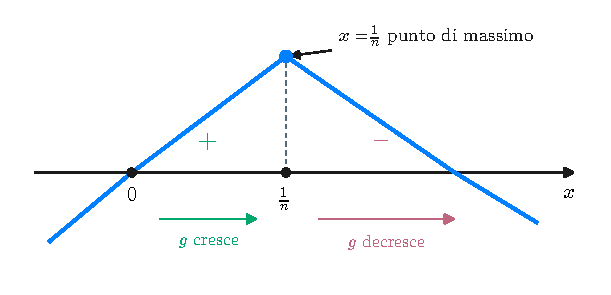
\includegraphics[width=0.82\textwidth]{immagini/segno_derivata}
\\[4pt]{\small\itshape Segno di $g'$ e andamento qualitativo di $g$ su $[0,+\infty[$.}
\end{center}

Quindi $g$ cresce su $[0, 1/n]$ e decresce su $[1/n, +\infty[$, e $x = 1/n$ è
punto di massimo assoluto (inoltre $g(0) = 0$ e $g(x) \to 0$ per
$x \to +\infty$). L'estremo superiore è un massimo e vale
\[
  M_n = g\!\left(\frac{1}{n}\right)
      = \frac{\dfrac{1}{n}}{1 + n^2 \cdot \dfrac{1}{n^2}}
      = \frac{1}{2n} \longrightarrow 0 .
\]

\paragraph{Conclusione.}
\[
  f_n \rightrightarrows 0 \quad \text{in } \mathbb{R} .
\]

% ---------------------------------------------------------------------
\needspace{12\baselineskip}
\subsection{Riepilogo}

\BoxBlue{Riepilogo del capitolo}{}{%
  \begin{itemize}
    \item Una successione di funzioni associa a ogni $n$ una funzione
          $f_n : I \to \mathbb{R}$; fissando $x$ si ottiene una successione numerica.
    \item \textbf{Convergenza puntuale}: $f_n(x) \to f(x)$ per ogni $x \in I$;
          l'indice $\nu$ dipende da $\varepsilon$ e da $x$.
    \item La convergenza puntuale \textbf{non} conserva la continuità
          ($x^n$ e $x^{1/n}$ su $[0,1]$).
    \item \textbf{Convergenza uniforme}: l'indice $\nu$ dipende solo da
          $\varepsilon$; graficamente, le $f_n$ entrano tutte nel tubo attorno a $f$.
    \item Criterio pratico:
          \[
            f_n \rightrightarrows f \text{ in } I
            \iff
            M_n = \sup_{x \in I} |f_n(x) - f(x)| \longrightarrow 0 .
          \]
    \item Uniforme $\Rightarrow$ puntuale, ma non viceversa: il limite uniforme,
          se esiste, è il limite puntuale.
    \item La convergenza uniforme dipende dall'insieme: spesso si ottiene
          restringendosi a insiemi limitati o allontanandosi dai punti di
          discontinuità del limite.
  \end{itemize}
}
